%%
%% This is file `elsarticle-template-num.tex',
%% generated with the docstrip utility.
%%
%% The original source files were:
%%
%% elsarticle.dtx  (with options: `numtemplate')
%% 
%% Copyright 2007, 2008 Elsevier Ltd.
%% 
%% This file is part of the 'Elsarticle Bundle'.
%% -------------------------------------------
%% 
%% It may be distributed under the conditions of the LaTeX Project Public
%% License, either version 1.2 of this license or (at your option) any
%% later version.  The latest version of this license is in
%%    http://www.latex-project.org/lppl.txt
%% and version 1.2 or later is part of all distributions of LaTeX
%% version 1999/12/01 or later.
%% 
%% The list of all files belonging to the 'Elsarticle Bundle' is
%% given in the file `manifest.txt'.
%% 

%% Template article for Elsevier's document class `elsarticle'
%% with numbered style bibliographic references
%% SP 2008/03/01

%\documentclass[preprint,12pt]{elsarticle}
\documentclass[preprint,10pt]{elsarticle}
%\documentclass[final,3p,times]{elsarticle} 

%% Use the option review to obtain double line spacing
%% \documentclass[authoryear,preprint,review,12pt]{elsarticle}

%% Use the options 1p,twocolumn; 3p; 3p,twocolumn; 5p; or 5p,twocolumn
%% for a journal layout:
%% \documentclass[final,1p,times]{elsarticle}
%% \documentclass[final,1p,times,twocolumn]{elsarticle}
%% \documentclass[final,3p,times]{elsarticle}
%% \documentclass[final,3p,times,twocolumn]{elsarticle}
%% \documentclass[final,5p,times]{elsarticle}
%% \documentclass[final,5p,times,twocolumn]{elsarticle}


\usepackage{array}
\usepackage{color}
\usepackage{graphicx}
\usepackage{float} % utiliser H pour forcer a mettre l'image ou on veut
\usepackage{mathbbol} % permet d'avoir le vrai symbol pour les reels grace a mathbb
\usepackage{stmaryrd} % permet d'utiliser \llbrackedt et \rrbracket : double crochet
\usepackage{subfigure}

%% The amssymb package provides various useful mathematical symbols 
%% The amsthm package provides extended theorem environments
\usepackage{amssymb}
\usepackage{amsmath}
% more math
\usepackage{amsfonts}
\usepackage{amssymb}
\usepackage{amstext}
\usepackage{amsbsy}


%% The lineno packages adds line numbers. Start line numbering with
%% \begin{linenumbers}, end it with \end{linenumbers}. Or switch it on
%% for the whole article with \linenumbers.
\usepackage{lineno}

\journal{TTSP}

\newcommand\bn{\boldsymbol{\nabla}}
\newcommand\bo{\boldsymbol{\Omega}}
\newcommand\br{\mathbf{r}}
\newcommand\la{\left\langle}
\newcommand\ra{\right\rangle}
\newcommand\bs{\boldsymbol}
\newcommand\red{\textcolor{red}}
\newcommand\ldb{\{\!\!\{}
\newcommand\rdb{\}\!\!\}}
\newcommand\llb{\llbracket}
\newcommand\rrb{\rrbracket}

\renewcommand{\(}{\left(}
\renewcommand{\)}{\right)}
\renewcommand{\[}{\left[}
\renewcommand{\]}{\right]}

\usepackage{setspace}
\newcommand{\tr}[1]{\textcolor{red}{#1}}
\newcommand{\tri}[1]{\textcolor{red}{{\it #1}}}

%%%%%%%%%%%%%%%%%%%%%%%%%%%%%%%%%%%%%%%%%%%%%%%%%%%%%%%%%%%%%%%%%%%%
% operators
\renewcommand{\div}{\vec{\nabla}\! \cdot \!}
\newcommand{\grad}{\vec{\nabla}}
% latex shortcuts
\newcommand{\bea}{\begin{eqnarray}}
\newcommand{\eea}{\end{eqnarray}}
\newcommand{\be}{\begin{equation}}
\newcommand{\ee}{\end{equation}}
\newcommand{\bal}{\begin{align}}
\newcommand{\eali}{\end{align}}
\newcommand{\bi}{\begin{itemize}}
\newcommand{\ei}{\end{itemize}}
\newcommand{\ben}{\begin{enumerate}}
\newcommand{\een}{\end{enumerate}}
% DGFEM commands
\newcommand{\jmp}[1]{[\![#1]\!]}                     % jump
\newcommand{\mvl}[1]{\{\!\!\{#1\}\!\!\}}             % mean value
\newcommand{\keff}{\ensuremath{k_{\textit{eff}}}\xspace}
% shortcut for domain notation
\newcommand{\D}{\mathcal{D}}
\newcommand{\J}{\mathcal{J}}
\newcommand{\I}{\mathcal{I}}
% vector shortcuts
\newcommand{\vo}{\vec{\Omega}}
\newcommand{\vr}{\vec{r}}
\newcommand{\vn}{\vec{n}}
\newcommand{\vnk}{\vec{\mathbf{n}}}
\newcommand{\vj}{\vec{J}}
% extra space
\newcommand{\qq}{\quad\quad}
% common reference commands
\newcommand{\eqt}[1]{Eq.~(\ref{#1})}                     % equation
\newcommand{\fig}[1]{Fig.~\ref{#1}}                      % figure
\newcommand{\tbl}[1]{Table~\ref{#1}}                     % table
\newcommand{\sct}[1]{Section~\ref{#1}}                   % section

\newcommand{\ud}{\,\mathrm{d}}
\newcommand{\mt}[1]{\marginpar{{\singlespacing \textcolor{red}{{\tiny #1}}}}}

%%%%%%%%%%%%%%%%%%%%%%%%%%%%%%%%%%%%%%%%%%%%%%%%%%%%%%%%%%%%%%%%%%%%%
%
%   BEGIN DOCUMENT
%
%%%%%%%%%%%%%%%%%%%%%%%%%%%%%%%%%%%%%%%%%%%%%%%%%%%%%%%%%%%%%%%%%%%%%
\begin{document}

%%%%%%%%%%%%%%%%%%%%%%%%%%%%%%%%%%%%%%%%%%%%%%%%%%%%%%%%%%%%%%%%%%%%
\begin{frontmatter}

%% Title, authors and addresses

%% use the tnoteref command within \title for footnotes;
%% use the tnotetext command for theassociated footnote;
%% use the fnref command within \author or \address for footnotes;
%% use the fntext command for theassociated footnote;
%% use the corref command within \author for corresponding author footnotes;
%% use the cortext command for theassociated footnote;
%% use the ead command for the email address,
%% and the form \ead[url] for the home page:
%\title{Title\tnoteref{label1}}
%% \tnotetext[label1]{}
%% \author{Name\corref{cor1}\fnref{label2}}
%% \ead{email address}
%% \ead[url]{home page}
%% \fntext[label2]{}
%% \cortext[cor1]{}
%% \address{Address\fnref{label3}}
%% \fntext[label3]{}

%-------------------------
%-------------------------
\title{Angular Multigrid Preconditioner for Krylov-based Solution Techniques
applied to the $S_n$ Equations with Highly Forward-Peaked Scattering}
\author{abc} 

\begin{abstract}
It is well known that diffusion synthetic acceleration (DSA) methods are ineffective 
when applied to the $S_n$ equations for problems with highly forward peak scattering. 
In \cite{multigrid_1d}, angular multigrid methods have been devised and proved to be 
significantly more effective for such problems (in one-dimensional space). 
The 1-D angular multigrid scheme is unconditionally stable, witrh a maximum spectral radius of $\sim0.6$
but extension of the method to multidimensional geometries can become unstable when the anisotropy is too
high. In \cite{multigrid_2d}, it was shown that diffusive filter is needed to stabilize the angular multigrid method;
however, this modified scheme results in spectral radii tending towards unity, making the technique ineffective.
Here, we recast angular multigrid method as a
preconditioner for a Krylov solver rather than using it as an acceleration
method for the Source Iteration technique applied to the $S_n$ equations. 
We show that the Krylov solver stabilizes the method and that filtering is no longer required. 
The new method is shown to be faster and
needs significantly fewer GMRES iterations than DSA preconditioning and sweep
preconditioning on two test problems. The eigenvalue spectra of the three
methods are compared. The proposed method gathers the eigenvalues and therefore, the
system requires fewer GMRES iterations to be solved.
\end{abstract}

%-------------------------
\begin{keyword}
aaa \sep
bbb.
\end{keyword}
%-------------------------
\end{frontmatter}
%-------------------------

%%%%%%%%%%%%%%%%%%%%%%%%%%%%%%%%%%%%%%%%%%%%%%%%%%%%%%%%%%%%%%%%%%%%
\linenumbers
\doublespacing

%%%%%%%%%%%%%%%%%%%%%%%%%%%%%%%%%%%%%%%%%%%%%%%%%%%%%%%%%%%%%%%%%%%%
%%%%%%%%%%%%%%%%%%%%%%%%%%%%%%%%%%%%%%%%%%%%%%%%%%%%%%%%%%%%%%%%%%%%
\section{Introduction}
%%%%%%%%%%%%%%%%%%%%%%%%%%%%%%%%%%%%%%%%%%%%%%%%%%%%%%%%%%%%%%%%%%%%
%%%%%%%%%%%%%%%%%%%%%%%%%%%%%%%%%%%%%%%%%%%%%%%%%%%%%%%%%%%%%%%%%%%%
Electron (and charged-particle) transport applications are ubiquitous and include radiotherapy, 
electronics hardening, etc. Charged particles interact through Coulomb
interactions with the background medium; each interaction results in only small changes and the particle's 
direction and energy. Such problems are characterized by highly forward peaked scattering kernels. 
In this paper, we consider the discrete-ordinate ($S_n$) angular discretization of the first-order form
of the transport equation. For many realistic problems, it is necessary to employ iterative solution 
techniques for the $S_n$ transport equations.  
%
If the scattering ratios $\(c_\ell=\frac{\Sigma_{s,\ell}}{\Sigma_t}\)$ (for $0 \le \ell \le N_a$, 
with $N_a$ the maximum anisotropy order in the cross-section data) is high, solving the $S_n$ transport
equations can be challenging due to the slow convergence of standard iterative algorithms, such as Source Iteration (SI). 
To speed up the convergence, acceleration schemes such as Diffusion
Synthetic Acceleration (DSA) must be used. DSA schemes focus on accelerating
the weakly anisotropic component of the angular flux moments (typically, only the zeroth or the zeroth and the first flux 
moments are accelerated \cite{adams}). While this is very efficient for neutron transport problems, for instance, it 
is inadequate for charged-particle transport \cite{multigrid_1d}. The spectral radius of the 
SI method accelerated with DSA becomes arbitrary close to one when the 
anisotropy increases and the scattering ratio is close to one. Even the use of optimized transport corrections for the scattering kernel
does not alleviate the ineffectiveness of DSA-accelerated SI schemes for highly forward peaked scattering problems \tri{need a REF}. 
\tri{also, should we be more explicit about the optimized TC? by saying something like: the scattering ratios are minimized?}
As a result, other methods have been 
developed to accelerate higher order angular flux moments 
\cite{multigrid_1d,multigrid_2d}. \tri{I think that you think that DSA is effective for flat modes in highly forward peaked problems, but it is not, even for these modes}\\
Morel and Manteuffel developed in \cite{multigrid_1d} an angular multigrid
method (ANMG) for the $S_n$ equations in one-dimensional geometry. Their angular
multigrid method uses a sequence of lower order transport operator and a
$P_1$ operator to accelerate higher moments. \tri{is the following statement you make true? that is, if no transport correction is applied, does ANMG fail, even in 1D? or is it that the transport correction is just more advantageous for 1D ANMG?} For the scheme to be able to
work, an ``optimal'' transport correction has to be applied to each transport
operator (in the context of angular multigrid, the optimal transport correction is done for each angular level). 
% the purpose of this correction is to minimize the scattering ratios of the angular moments that are not accelerated
This transport correction minimizes the ``high-frequency'' angular
errors. Their results were very encouraging; Pautz and Adams generalized the ANMG method 
to multidimensional geometries \cite{multigrid_2d}. This multidimensional
extension of the original angular multigrid method needs to be stabilized
because the scheme amplifies the high-frequency error modes
instead of damping them.\tri{can you give more details? I think it is the corrections to the high-frequency modes that are being messed up by ANMG}  
They proposed a 
filter which allows the scheme to be always stable but which also reduces the 
efficiency of the method compared to the one dimensional case. Consequently, the spectral 
radius of the filtered-ANMG method can become arbitrary close to one when the anisotropy increases.\\

The angular multigrid methods proposed so far were only applied in the context
of a SI solution technique. However, the underlying linear system of equations 
can also be tackled using non-stationary 
Krylov solvers, such as GMRES. In \cite{ttg}, the authors applied GMRES to
the single group $S_n$ equations with isotropic scattering and 
summarized the advantageous features of GMRES as follows~: ``using DSA as a 
preconditioner for GMRES(m) removes the consistency requirement that plagues 
DSA-accelerated source iteration in multidimensional problems.'' 
\tri{your quote of their work deals with the consistency issue of the spatial discretization;
what we would like to emphasize here is : (1) DSA-accelerated SI can be recast as preconditioned GMRES,
(2) it is effective, even when the SI+DSA scheme is not effective due to the partially consistent DSA discretization, (3) there, we 
hope that GMRES where ANMG is the preconditioner will be effective, hopefully WITHOUT the need for the filtered version of ANMG}
Driven by this
property, we propose to use the angular multigrid as a preconditioner for a 
Krylov solver instead of an acceleration scheme for the Source Iteration
method with application to problems with highly forward-peaked scattering. 
The Krylov solver does not require the method to have a spectral
radius below one to be effective and, therefore, the filter used in
\cite{multigrid_2d} becomes
unnecessary. Furthermore, a code solving the $S_n$ equations using SI with DSA can easily
be modified to use a preconditioned Krylov solver. \\

In this work, we introduce some notations and recall iterative solution techniques applied 
to the $S_n$ transport equations in \sct{sec:sn_eqs} and \sct{sec:sn_iterative_review}. 
In \sct{sec:previous_anmg}, we review the previous work on the ANMG method applied to SI in one-dimensional and multi-dimensional spaces.
Next, we propose in \sct{sec:anmg_krylov} to re-formulate the SI+ANMG technique as a preconditioner for a Krylov solver (GMRES).
\tri{is there was value in presenting ANMG where the coarsest level is DSA {\bf AND}  ANMG where the coarsest level is P1SA? This is what is in this section currently and I am uncertain about what to do with this yet}. 
Results are presented in \sct{sec:results} and we show some results and we end with some conclusions in \sct{sec:ccl}.

%-------------------------
%%%%%%%%%%%%%%%%%%%%%%%%%%%%%%%%%%%%%%%%%%%%%%%%%%%%%%%%%%%%%%%%%%%%%%%%%%%%%%%%%%%%
%%%%%%%%%%%%%%%%%%%%%%%%%%%%%%%%%%%%%%%%%%%%%%%%%%%%%%%%%%%%%%%%%%%%%%%%%%%%%%%%%%%%
\section{Review of iterative solution techniques applied to the $S_n$ transport equation}
%%%%%%%%%%%%%%%%%%%%%%%%%%%%%%%%%%%%%%%%%%%%%%%%%%%%%%%%%%%%%%%%%%%%%%%%%%%%%%%%%%%%
%%%%%%%%%%%%%%%%%%%%%%%%%%%%%%%%%%%%%%%%%%%%%%%%%%%%%%%%%%%%%%%%%%%%%%%%%%%%%%%%%%%%

\tri{why even bother with multigroup? just say the eqs are typically discrete in energy groups, you may want to cite CEPXs for
where XS typically come from in deterministic codes. After that, I would just give the one-group eqs. Also, I would prepare the Readers at this point that the XS we have chosen for our example are of FP-type and you can cite a couple of references, Morel and Pautz for example, where they employ FP scattering as a model of highly forward peaked scattering and use it in 1-g calculations to do proof-of-principle stuff}.

In this section, we first give the multigroup $S_n$ transport equations. Next,
the Source Iteration technique is recalled and the $S_n$ equations are
recast to be solved by a Krylov solver. Previous work on angular
multigrid methods applied as preconditioner to SI is presented. Finally, we
conclude this section with the derivation of the new method.  

%%%%%%%%%%%%%%%%%%%%%%%%%%%%%%%%%%%%%%%%%%%%%%%%%%%%%%%%%%%%%%%%%%%%%%%%%%%%%%%%%%%%
\subsection{Multigroup $S_n$ equations} \label{sec:sn_eqs}
%%%%%%%%%%%%%%%%%%%%%%%%%%%%%%%%%%%%%%%%%%%%%%%%%%%%%%%%%%%%%%%%%%%%%%%%%%%%%%%%%%%%
\tri{this sections deals mostly with sn eqs, notation, and FP scattering as an example kernel. this title of this section must reflect this}

Charged particles transport can be described by the Boltzmann equation
\cite{graal} which discretized in energy using the standard multigroup method
\cite{reuss} and in angle using the discrete ordinate method \cite{reuss}, is
given by :
\begin{equation}
\bo_d \cdot \bn \Psi_d^g(\br) + \Sigma_{t,g}^g(\br) \Psi_d^g(\br) = \sum_{g'=0}^G
\sum_{l=0}^L\sum_{m=-l}^l \frac{2l+1}{4\pi}\Sigma_{s,l}^{g'\rightarrow
g}\Phi_{l,m}^{g'}(\br)Y_l^m(\bo_d) + Q_d^g(\br)
\label{discretized}
\end{equation}
where $\br$ is the position in domain $\mathcal{D}$, $E$ is the energy,
$\bo_d=(\mu_d,\varphi_d)$, $\mu_d$ is the cosine of the directional polar angle,
$\varphi_d$ is the directional azimuthal angle, 
$\Psi_d^g(\br)=\int_{E^{g}}^{E^{g-1}}\Psi(\br,\bo_d,E)\ dE$, $\Psi$ is
the angular flux, $Q_d^g(\br) = \int_{E^g}^{E^{g-1}}Q(\br,\bo_d,E) dE$, $Q$ is
a volumetric source, $\Sigma_{t}^g(\br)$ is the multigroup total 
macroscopic cross section, $\Sigma_{s,l}$ is the Legendre moment of 
degree $l$ of $\Sigma_s$ and $\Phi_{l,m}(\br,E)= \int_{4\pi}\Psi(\br,\bo,E)Y_l^{m,*}(\bo)\ d\bo
\approx \sum_{d=1} w_d \Psi(\br,\bo_d,E)Y_l^{m,*}(\bo_d)$ where $Y_l^m$ 
are the spherical harmonics.
Standard boundary conditions can be applied to (\ref{discretized}); the most
commonly employed is the incoming flux boundary condition :
\begin{equation}
\Psi(\br,\bo,E) = g(\br,\bo,E)\textrm{ for }\bo\cdot\bs{n}<0\textrm{ and
}\br\in \partial \mathcal{D},
\label{boundary}
\end{equation} 
where $\partial \mathcal{D}$ is the boundary of the domain $\mathcal{D}$. If $g=0$, equation
(\ref{boundary}) yields vacuum boundary conditions.\\
This equation still needs to be discretized in space but the method proposed
in this paper is not restricted to a particular spatial discretization. For
the results presented here, we use bilinear discontinuous finite elements in
two dimensional space problem \cite{dgfem}.\\ 
Equation (\ref{discretized}) can be written using operator notation as :
\begin{equation}
L \bs{\Psi} = M\Sigma D \bs{\Psi} + \bs{Q}
\label{operator}
\end{equation}
where $\bs{\Psi}$ is a vector containing all the $\Psi_d$, $\bs{Q}$ is a
vector containing all the $Q_d$, $\Sigma$ is a diagonal matrix with the
element $\Sigma_{s,l}$ as diagonal elements, $M$ is the moment-to-discrete
matrix $(\bs{\Psi} = M\bs{\Phi})$, $D$ is the discrete-to-moments matrix
$(\Phi=D\Psi)$ (the moment entries are dictated  by the dimensionality of the
problem) and $L = \bo\cdot + \Sigma_t$ is the streaming + total interaction operator,
inverted direction by direction (transport sweeps). The inversion can be done
locally for each mesh cell for each discrete directional fluxes in the
quadrature.\\
The cross section used here are the Fokker-Planck cross sections :
\begin{equation}
\Sigma_{s,l}=\frac{\alpha}{2} (L(L+1)-l(l+1))\ \ l=0,\hdots,L
\end{equation}
where $\alpha$ is the restricted momentum transfer \cite{morel_96}.
These cross sections approximate the electron scattering cross sections
\cite{morel_81} and require Galerkin quadratures , i.e.,
$D=M^{-1}$ \cite{graal}, to obtain accurate results.


%%%%%%%%%%%%%%%%%%%%%%%%%%%%%%%%%%%%%%%%%%%%%%%%%%%%%%%%%%%%%%%%%%%%%%%%%%%%%%%%%%%%
\subsection{Solution Techniques} \label{sec:sn_iterative_review}
%%%%%%%%%%%%%%%%%%%%%%%%%%%%%%%%%%%%%%%%%%%%%%%%%%%%%%%%%%%%%%%%%%%%%%%%%%%%%%%%%%%%

Equation (\ref{operator}) can be solved using the Source Iteration method or a
Krylov method. The Source Iteration method at the $k^{th}$ iteration is given
by :
\begin{equation}
\bs{\Phi}^{(k+1)} = DL^{-1}M\Sigma \bs{\Phi}^{(k)} + DL^{-1}\bs{Q}
\end{equation}
\tri{careful, not just $c_0$ but $c_\ell$}
The spectral radius of SI can become arbitrary close to one when the
scattering ratio $\(\frac{\Sigma_{s,0}}{\Sigma_t}\)$ is close to one. 
To accelerate the convergence of SI, the Diffusion Synthetic
Acceleration scheme \cite{adams} is commonly used. The SI+DSA scheme is given by :
\begin{align}
&\bs{\Phi}^{(k+1/2)} = DL^{-1}M\Sigma\bs{\Phi}^{(k)} + DL^{-1}\bs{Q}\\
&\delta\bs{\Phi}^{(k)} = \mathcal{T}_0^{-1} R_{n\rightarrow 0} 
\(\bs{\Phi}^{(k+1/2)}-\bs{\Phi}^{(k)}\)\\
&\bs{\Phi}^{(k+1)} = \bs{\Phi}^{(k+1/2)} + P_{0/1 \rightarrow n} \delta
\bs{\Phi}^{(k)}
\end{align}
Finally, we get :
\begin{equation}
\bs{\Phi}^{(k+1)} = \((I+P_{0/1\rightarrow n} \mathcal{T}_0^{-1} R_{n\rightarrow 0} )
DL^{-1}M\Sigma-P_{0/1\rightarrow n}\mathcal{T}_0^{-1} R_{n\rightarrow 0}\)
\bs{\Phi}^{(k)} + (I+P_{0/1\rightarrow n}\mathcal{T}_0^{-1}
R_{n\rightarrow 0})DL^{-1} Q
\end{equation}
where $\mathcal{T}_0$ is the DSA operator, $R_{n\rightarrow 0}$ is the
restriction matrix of $\bs{\Phi}_{n}$ to $\bs{\Phi}_0$ and $P_{0/1 \rightarrow
n}$ is the projection matrix of $\bs{\Phi}_0$ or $\bs{\Phi}_1$, depending
whether only the zeroth or the zeroth and the first moment are accelerated, to
$\bs{\Phi}_n$.\\
When using a Krylov solver, equation (\ref{operator}) has to be rewritten as :
\begin{equation}
(I-DL^{-1}M\Sigma) \bs{\Phi} = DL^{-1}\bs{Q}
\label{krylov}
\end{equation}
where $I$ is the identity matrix. Equation (\ref{krylov}) is equation
(\ref{operator}) preconditioned by $DL^{-1}$ (sweep preconditioning). DSA can also 
help to speed up the convergence of the Krylov solver. The system of equations 
solved with the Krylov method is :
\begin{equation}
\((I+P_{0/1 \rightarrow n}\mathcal{T}_0^{-1} R_{n\rightarrow 0})(I-DL^{-1}M\Sigma)\)
\bs{\Phi} = (I+P_{0/1 \rightarrow n}\mathcal{T}_0^{-1} R_{n\rightarrow 0})DL^{-1}Q
\end{equation}       

%%%%%%%%%%%%%%%%%%%%%%%%%%%%%%%%%%%%%%%%%%%%%%%%%%%%%%%%%%%%%%%%%%%%%%%%%%%%%%%%%%%%
\subsection{Review of Previous Angular Multigrid Work} \label{sec:previous_anmg}
%%%%%%%%%%%%%%%%%%%%%%%%%%%%%%%%%%%%%%%%%%%%%%%%%%%%%%%%%%%%%%%%%%%%%%%%%%%%%%%%%%%%

\subsubsection{One dimensional geometry}
%%%%%%%%%%%%%%%%%%%%%%%%%%%%%%%%%%%%%%%%%%%%%%%%%%%%%%%%%%%%%%%%%%%%%%%%%%%%%%%%%%%%

As mentioned previously, only the zeroth and the first flux moments can be
accelerated with DSA. To accelerate higher moments, other methods have to be
used. Morel and Manteuffel have proposed an angular 
multigrid method to accelerate the inner SI calculation of the one dimension 
$S_n$ equations when the scattering is highly anisotropic 
\cite{multigrid_1d}. The motivation to use a variation of the extended
transport correction \cite{lathrop} to attenuate the ``upper half'' of the
flux moments (higher frequencies) thanks to transport sweeps. The ``lower half'' 
of the flux moments (lower frequencies) is accelerated using the $S_{n/2}$ 
equations. These $S_{n/2}$ equations are themselves 
accelerated using $S_{n/4}$ equations. The order of the transport operator is 
divided by two 
until the $S_4$ equations are solved. At this point, the $P_1$ equations are 
used to accelerate the $S_4$ equations. We define :
\tri{for the unfamiliar reader, give a short explanation for the definition of Half. It is because 
S8-S4-S2 works great, but if one starts with S6, there are no S3, so it is S6-S4-S2. I think these examples are worthwhile}
\begin{equation}
Half(n) = \left\{
\begin{aligned}
&\frac{n}{2}, &\textrm{if $\frac{n}{2}$ is even}\\
&\frac{n}{2}+1, &\textrm{if $\frac{n}{2}$ is odd}
\end{aligned}
\right.
\end{equation}
Their scheme works as follows : 
\begin{enumerate}
\item Perform a transport sweep for the $S_n$ equations.
\item Perform a transport sweep for the $S_{n_2}$ equations with a $P_{n_2-1}$
expansions using the $S_n$ residual as the inhomogeneous source, where
$n_2=Half(n)$.
\item Continue coarsening the angular grid by a factor two (i.e., according to
the definition of ``$Half$'') until a sweep has been performed for the $S_4$
equations.
\item Solve the $P_1$ equations (P1SA) with a $P_1$ expansion of the $S_4$
residual as the inhomogeneous source.
\item Add the Legendre moments of the diffusion solution to the Legendre
moments of the $S_4$ iterate to obtain the accelerated $S_4$ iterate.
\item Continue to add the corrections from each coarse grid to the finer grid
above to obtain the accelerated $S_n$ moments.
\end{enumerate}
Every time a transport sweep is performed, the optimal transport correction
needs to be used \cite{multigrid_1d}. For a $P_{n-1}$ expansion of the cross
sections, the corrected cross sections are given by :
\begin{equation}
\Sigma_{j}^* = \Sigma_{j} -\frac{\Sigma_{s,n/2}+\Sigma_{s,n-1}}{2}\ 
\textrm{ with }j=t \textrm{ or }s,l
\end{equation}
This correction is said to be optimal because for an infinite homogeneous medium, 
it minimizes the ``high-frequency'' angular errors, the smoothing factor being 
given by :
\begin{equation}
\rho_s =
\max(|\Sigma_{s,n/2}|/\Sigma_{s,0},|\Sigma_{s,n/2+1}|/\Sigma_{s,0},\hdots,
|\Sigma_{s,n-1}|/\Sigma_{s,0})
\end{equation}
To compare the effectiveness of the angular multigrid method with DSA, 
Fokker-Planck scattering cross sections can be used. In one dimension,
DSA becomes less efficient as $\Sigma_{s,l}$ $(l>0)$ becomes closer to
$\Sigma_{s,0}$. Therefore, in the limit as $L\rightarrow \infty$, DSA no
longer accelerates the convergence of SI when Fokker-Planck cross section are used. 
The spectral radius tends to 1.0 and thus,
the acceleration scheme is inefficient. However, the spectral radius of the
angular multigrid method has an upper bound of 0.6 when $L$ goes to
infinity.


\subsubsection{Extension to multidimensional geometries}
%%%%%%%%%%%%%%%%%%%%%%%%%%%%%%%%%%%%%%%%%%%%%%%%%%%%%%%%%%%%%%%%%%%%%%%%%%%%%%%%%%%%

In the multidimensional case, DSA becomes unstable when both the zeroth
and the first flux moments are accelerated and $\frac{\Sigma_{s,1}}{\Sigma_t}
\geq 0.5$ \cite{multisweep}. In \cite{multigrid_2d}, the authors modified the
one dimensional angular multigrid method by accelerating only the zeroth flux
moment with the DSA and by using $S_2$ as lowest transport sweep
instead of an $S_4$. Moreover, a
filter is now needed to stabilize the method. Therefore, the angular multigrid 
method was modified as follows \cite{multigrid_2d} :
\begin{enumerate}
\item Perform a transport sweep for the $S_n$ equations.
\item Perform a transport sweep for the $S_{n_2}$ equations with a $P_{n_2}$
for 2-D problem and a $P_{n_2+1}$ for 3-D problem expansion for the $S_n$
residual as the inhomogeneous source, where $n_2=Half(n)$.
\item Continue coarsening the angular grid by a factor two (i.e., according to the
definition of ``$Half$'') until a sweep has been performed for the $S_2$
equations.
\item Solve the diffusion equation with a $P_0$ expansion for the $S_2$
residual as the inhomogeneous source. 
\item Apply a diffusive filter to the corrections from steps 2 and 3 (without
this filter, the method is unstable).
\item Add the corrections from steps 4 and 5 to the Legendre moments of the
$S_n$ iterate to obtain the accelerated $S_n$ moments.
\end{enumerate}
The filter stabilizes the method which otherwise would diverge but it reduces
the efficiency of the angular multigrid. The spectral radius can become
arbitrary close to one when $L$ becomes large \cite{multigrid_2d}.


%%%%%%%%%%%%%%%%%%%%%%%%%%%%%%%%%%%%%%%%%%%%%%%%%%%%%%%%%%%%%%%%%%%%%%%%%%%%%%%%%%%%
%%%%%%%%%%%%%%%%%%%%%%%%%%%%%%%%%%%%%%%%%%%%%%%%%%%%%%%%%%%%%%%%%%%%%%%%%%%%%%%%%%%%
\section{Angular Multigrid as a Preconditioner for Krylov Solvers} \label{sec:anmg_krylov}
%%%%%%%%%%%%%%%%%%%%%%%%%%%%%%%%%%%%%%%%%%%%%%%%%%%%%%%%%%%%%%%%%%%%%%%%%%%%%%%%%%%%
%%%%%%%%%%%%%%%%%%%%%%%%%%%%%%%%%%%%%%%%%%%%%%%%%%%%%%%%%%%%%%%%%%%%%%%%%%%%%%%%%%%%

In this paper, we propose to abandon SI as the solver for the $S_n$ equations 
and to use the angular multigrid method as a preconditioner for the Krylov solver. 
The successive corrections of the angular multigrid acceleration form
now different stages of a preconditioner used int the Krylov solver. Since, a Krylov solver is used to
stabilize the method, two variations are possible :
\begin{itemize}
\item the coarsest level can be DSA (ANMG-DSA).
\item the coarsest level can be P1SA (ANMG-P1SA).
\end{itemize}
First, we present the angular multigrid using DSA and then, the angular
multigrid using P1SA. Later, these two versions are be compared.

%%%%%%%%%%%%%%%%%%%%%%%%%%%%%%%%%%%%%%%%%%%%%%%%%%%%%%%%%%%%%%%%%%%%%%%%%%%%%%%%%%%%
\subsection{ANMG-DSA}
%%%%%%%%%%%%%%%%%%%%%%%%%%%%%%%%%%%%%%%%%%%%%%%%%%%%%%%%%%%%%%%%%%%%%%%%%%%%%%%%%%%%

Using a method similar to the one we used to write the equation for the 
preconditioned Krylov solver, we obtain \hbox{successively :}
\begin{align}
& \Phi_n^{(k+1/2)} = D_n L_n^{-1} M_n \Sigma_n \Phi_n^{(k)} + D_n L_n^{-1} Q\\
& \delta \Phi_{n/2}^{(k)} = D_{n/2} L_{n/2}^{-1} M_{n/2} \Sigma_{n/2}
R_{n\rightarrow n/2} \(\Phi_n^{(k+1/2)}-\Phi_n^{(k)}\)\\
& \hdots\\
& \delta \Phi_2^{(k)} = D_2 L_2^{-1} M_2 \Sigma_2 R_{4\rightarrow 2} \delta \Phi_4\\
& \delta \Phi_0^{(k)} = \mathcal{T}_0^{-1} R_{2\rightarrow 0} \delta \Phi_2^{(k)} \\
& \Phi_n^{(k+1)} = \Phi_n^{(k+1/2)} + P_{n/2 \rightarrow n} \delta
\Phi_{n/2}^{(k)} + \hdots + P_{2 \rightarrow n} \delta \Phi_{2}^{(k)} + P_{0
\rightarrow n} \delta \Phi_{0}^{(k)}
\end{align}

\begin{equation}
\begin{split}
\Phi_n^{(k+1)} =& T_n \Phi_n^{(k)} + D_n L_n^{-1} Q +
P_{n/2 \rightarrow n} \(T_{n/2}
R_{n\rightarrow n/2} \(\Phi_n^{(k+1/2)} - \Phi_n^{(k)}\)\)+\hdots \\
&+ P_{2 \rightarrow n} T_2 R_{4\rightarrow 2} \delta
\Phi_{4}^{(k)} + P_{0\rightarrow n} \mathcal{T}_0^{-1} R_{2\rightarrow 0} \delta 
\Phi_2^{(k)}\\
=& T_n \Phi_n^{(k)} + D_n L_n^{-1} Q + P_{n/2 \rightarrow
n} \(T_{n/2} R_{n \rightarrow n/2}\(T_n \Phi_n^{(k)} +D_n L_n^{-1} Q -\Phi_n^{(k)}
\)\)\\
& +\hdots + P_{2\rightarrow n} T_2 R_{4\rightarrow 2} 
\(T_4 R_{8\rightarrow 4}\( \hdots \(T_n \Phi_n^{(k)} + D_n L_n^{-1} Q -
 \Phi_n^{(k)}\)\) \) \\ 
&+ P_{0\rightarrow n} \mathcal{T}_0^{-1} R_{2\rightarrow 0}\(T_2 R_{4\rightarrow 2} 
\(\hdots\(T_n \Phi_n^{(k)}+D_n L_n^{-1}Q-\Phi_n^{(k)}\)\)\)\\
=& \(T_n + P_{n/2\rightarrow n} T_{n/2} R_{n\rightarrow n/2}\(T_n-I\)+
 \hdots + P_{2\rightarrow n} T_2 R_{4\rightarrow}
\(T_4 R_{8\rightarrow 4} \(\hdots\(T_n -I\)\)\)\right.\\ 
&\left. +P_{0\rightarrow n} \mathcal{T}_0^{-1} R_{2\rightarrow 0}  \(T_2
R_{4\rightarrow 2} (\hdots \(T_n-I\))\)\) \Phi_n^{(k)}
+\(I+P_{n/2\rightarrow n} T_{n/2} R_{n\rightarrow
n/2}+ \hdots + \right.\\
&\left. P_{2\rightarrow n} T_2 R_{4\rightarrow 2} \(T_4
 R_{8\rightarrow 4}\(\hdots
\(T_{n/2}R_{n\rightarrow n/2}\)\)\)+\right.\\
& \left. P_{0\rightarrow n} \mathcal{T}_0^{-1}R_{2\rightarrow 0}
\(T_2 R_{4\rightarrow 2}\(\hdots\(T_{n/2}R_{n\rightarrow n/2}\)\)\)\)
D_nL_n^{-1} Q
\end{split}
\end{equation}
where $T_n = D_n L_n^{-1}M_n \Sigma_n$. We use the subscript $n$ as a reminder
that we are solving the $S_n$ equations.\\
Finally, the system of equations which has to be solved is :
\begin{equation}
\begin{split}
&(I+P_{{n}/{2}\rightarrow n }
T_{{n}/{2}} (I+P_{{n}/{4}\rightarrow {n}/{2}}T_{{n}/{4}} (\hdots
(I+P_{0\rightarrow 2} \mathcal{T}_0^{-1} R_{2\rightarrow 0})\hdots)
R_{{n}/{2}\rightarrow {n}/{4}})R_{n\rightarrow{n}/{2}})(I-T_n)
\bs{\Phi}_n =\\
& (I+P_{{n}/{2}\rightarrow n} T_{{n}/{2}} (I+P_{{n}/{4}
\rightarrow {n}/{2}} T_{{n}/{4}} (\hdots (I+P_{0 \rightarrow
2}\mathcal{T}_0^{-1} R_{2\rightarrow 0})\hdots)R_{{n}/{2}\rightarrow
{n}/{4}})R_{n\rightarrow {n}/{2}} ) D_n L_n^{-1} Q
\end{split}
\label{anmg-dsa}
\end{equation}  
At this point, it is necessary to choose a DSA scheme. Among different
schemes (see \cite{adams}), the Modified Interior Penalty (MIP) DSA was
chosen \cite{mip}. This DSA is based on a second-order discontinuous of a
diffusion equation, as opposed to a mixed of $P1$ formulation.
It uses bilinear discontinuous finite elements, which is
the same spatial discretization that the one chosen for the
$S_n$ equations and it has been shown to be always stable for isotropic
scattering and is symmetric positive definite (SPD), which makes it easy to invert.
We will recall here the weak form of this DSA :
\begin{equation}
b_{MIP}(\phi,\phi^*) = l_{MIP}(\phi^*)
\end{equation}
with :
\begin{equation}
\begin{split}
b_{MIP}(\phi,\phi^*) =& (\Sigma_a \phi,\phi^*)_{\partial D} +
\(\mathrm{D}\bn\phi,\bn\phi^*\)_{\mathcal{D}} + \(\kappa_e\llb\phi\rrb,
\llb\phi^*\rrb\)_{E_h^i}
+ \(\llb\phi\rrb,\ldb \mathrm{D}\partial_n \phi^*\rdb\)_{E_h^i} +\\
&(\ldb \mathrm{D} \partial_n \phi\rdb,\llb\phi^*\rrb)_{E_h^i} + 
(\kappa_e\phi,\phi^*)_{\partial
D^d}-\frac{1}{2} \(\phi,\mathrm{D}\partial_n \phi^*\)_{\partial
\mathcal{D}^d} - \frac{1}{2} (\mathrm{D} \partial_n \phi,\phi^*)_{\partial 
\mathcal{D}^d}
\end{split}
\end{equation}
\begin{equation}
l_{MIP}(\phi^*) = (Q_0,\phi^*)_{\mathcal{D}} 
\end{equation}
where :
\begin{itemize}
\item $(f,g)_{\mathcal{D}} = \sum_{K\in \mathbb{T}_h} \int_K fg\ d\br$ and 
$(f,g)_{E_h^i} = \sum_{e\in E_h^i} \int_e fg\ ds$
\item $\mathbb{T}_h$ is the mesh used to discretize the domain $\mathcal{D}$
into nonoverlapping elements $K$, $E_h^i$ is the set of interior edges,
$\mathcal{D}$ is the spatial domain, $\partial \mathcal{D}^d$ is the boundary
of the domain with Dirichlet condition and $\partial \mathcal{D}^r$ is the
boundary of the domain with reflective condition
\item $\Sigma_a$ is the absorption macroscopic cross section
\item $\mathrm{D}$ is the diffusion coefficient
\item $\partial_n = \bs{n}\cdot \bn$ where $\bs{n}$ is the outward unit
normal
\item $\llb \phi\rrb = \phi^{+}-\phi^{-}$ is the jump of at the interface
between two elements
\item $\ldb\phi\rdb = \frac{\phi^++\phi^-}{2}$ is the mean of $\phi$ at the
interface between two elements
\item $\phi^{\pm}(\br)=\lim_{s\to 0^{\pm}}\phi(\br+s\bs{n}_e)$, $\bs{n}_e$ is
the normal unit vector associated with a given edge $e$
\item $\kappa_e = \max\(\kappa_e^{IP},\frac{1}{4}\)$ with
$\kappa_e^{IP}=\left\{
\begin{aligned}
&\frac{c(p^+)}{2}\frac{D^+}{h_{\bot}^+} + \frac{c(p^-)}{2}
\frac{D^-}{h_{\bot}^-} &\textrm{ on interior edges, i.e. }e\in E_h^i\\
&c(p)\frac{D}{h_{\bot}} & \textrm{ on boundary edges,
i.e. }e\in\partial\mathcal{D}^d
\end{aligned}
\right.$\\
$c(p)$ is given by $c(p)=2p(p+1)$, $p$ is the polynomial order and $h_{\bot}$
is the length of the cell in the direction orthogonal to the edge $e$
\end{itemize}

%%%%%%%%%%%%%%%%%%%%%%%%%%%%%%%%%%%%%%%%%%%%%%%%%%%%%%%%%%%%%%%%%%%%%%%%%%%%%%%%%%%%
\subsection{ANMG-P1SA}
%%%%%%%%%%%%%%%%%%%%%%%%%%%%%%%%%%%%%%%%%%%%%%%%%%%%%%%%%%%%%%%%%%%%%%%%%%%%%%%%%%%%

Using P1SA and $S_4$ as the lowest $S_n$ order instead of DSA and $S_2$ in 
equation (\ref{anmg-dsa}) gives us :
\begin{equation}
\begin{split}
& (I+P_{n/2\rightarrow n} T_{n/2} (I+P_{n/4\rightarrow n/2}
T_{n/4}(\hdots(I+P_{1\rightarrow 4}\mathcal{T}_1^{-1} R_{4\rightarrow
1})\hdots)R_{n/2 \rightarrow n/4})R_{n\rightarrow n/2}) (I-T_n)\bs{\Phi}_n = \\
& (I+P_{n/2\rightarrow n} T_{n/2} (I+P_{n/4\rightarrow n/2}
T_{n/4}(\hdots(I+P_{1\rightarrow 4}\mathcal{T}_1^{-1} R_{4\rightarrow
1})\hdots)R_{n/2\rightarrow n/4})R_{n\rightarrow n/2}) D_n L_n^{-1} Q
\end{split}
\end{equation}
where $\mathcal{T}_1$ is the P1SA operator.\\
The P1SA used is the P1C defined in \cite{yaqi}. This scheme,
which is positive definite but non-symmetric, is given by :
\begin{equation}
b_{P1C}(\Phi,\bs{J},\Phi^*,\bs{J}^*) = l_{P1C}(\Phi^*,\bs{J}^*)
\end{equation}
with :
\begin{equation}
\begin{split}
b_{P1}(\Phi,\bs{J},\Phi^*,\bs{J}^*) = & (\Sigma_a \Phi,\Phi^*)_{\mathcal{D}} +
(3\Sigma_{tr} \bs{J},\bs{J}^*)_{\mathcal{D}} + (\bn
\Phi,\bs{J}^*)_{\mathcal{D}} - (\bs{J},\bn \Phi^*)_{\mathcal{D}}\\
&+\frac{1}{4} \(\llb\Phi\rrb,\llb\Phi^*\rrb\)_{E_h^i} +
\(\llb\Phi\rrb,\ldb\bs{J}\cdot\bs{n}_e\rdb\)_{E_h^i} - (\ldb
\bs{J}\cdot\bs{n}_e\rdb, \llb\Phi^*\rrb)_{E_h^i}\\
&+\frac{9}{16}\(\llb\bs{J}\cdot\bs{n}_e\rrb,\llb\bs{J}^*\cdot\bs{n}_e\rrb\)_{E_h^i}
+ \frac{9}{16}\(\llb\bs{J}\rrb,\llb\bs{J}^*\rrb\)_{E_h^i}\\
&+\frac{1}{4}(\Phi,\Phi^*)_{\partial \mathcal{D}^d} +
\frac{1}{2}(\Phi,\bs{J}^*\cdot\bs{n}_e)_{\partial \mathcal{D}^d} - \frac{1}{2}
(\bs{J}\cdot\bs{n}_e,\Phi^*)_{\partial\mathcal{D}^d}\\
&+\frac{9}{16}(\bs{J},\bs{J}^*)_{\partial
\mathcal{D}^d}+\frac{9}{16}(\bs{J}\cdot\bs{n}_e,\bs{J}^*\cdot\bs{n}_e)_{\partial 
\mathcal{D}^d} + \frac{9}{4} (\bs{J}\cdot\bs{n}_e,\bs{J}^*\cdot\bs{n}_e)_{\partial
\mathcal{D}^r}
\end{split}
\end{equation}
\begin{equation}
l(\Phi^*,\bs{J}^*) = (Q_0,\Phi^*)_{\mathcal{D}} +
(3\bs{Q}_1,\bs{J}^*)_{\mathcal{D}}
\end{equation}
where $\bs{J}$ is the current or first moment of the flux and 
$\Sigma_{tr}=\Sigma_t-\Sigma_{s,1}$.

%-------------------------
%%%%%%%%%%%%%%%%%%%%%%%%%%%%%%%%%%%%%%%%%%%%%%%%%%%%%%%%%%%%%%%%%%%%%%%%%%%%%%%%%%%%
%%%%%%%%%%%%%%%%%%%%%%%%%%%%%%%%%%%%%%%%%%%%%%%%%%%%%%%%%%%%%%%%%%%%%%%%%%%%%%%%%%%%
\section{Results} \label{sec:results}
%%%%%%%%%%%%%%%%%%%%%%%%%%%%%%%%%%%%%%%%%%%%%%%%%%%%%%%%%%%%%%%%%%%%%%%%%%%%%%%%%%%%
%%%%%%%%%%%%%%%%%%%%%%%%%%%%%%%%%%%%%%%%%%%%%%%%%%%%%%%%%%%%%%%%%%%%%%%%%%%%%%%%%%%%

In this section, we first compare the number of GMRES iteration needed by 
ANMG-DSA and ANMG-P1SA to solve a test case. Then, both the number of GMRES 
iterations and the elapsed time are compared for three methods :
\begin{itemize}
\item Sweep preconditioning (S).
\item DSA with optimal transport correction preconditioning (DSA).
\item Angular multigrid with DSA preconditioning (ANMG-DSA).
\end{itemize}
The tests use a homogeneous medium and Fokker-Planck cross
sections with $\alpha=1$. $\Sigma_{t}$ is chosen to be equal to
$\Sigma_{s,0}$. The quadrature is the Gauss-Legendre-Chebyshev Galerkin
quadrature. The domain is a $5cm$ side square and the uniform mesh is composed
of 50 by 50 
cells. The GMRES solver is converged to a relative tolerance of $10^{-4}$. To
conclude this section, the eigenvalue spectrum of the three methods is
compared on a example.

%%%%%%%%%%%%%%%%%%%%%%%%%%%%%%%%%%%%%%%%%%%%%%%%%%%%%%%%%%%%%%%%%%%%%%%%%%%%%%%%%%%%
\subsection{Comparison between ANMG-DSA and ANMG-P1SA}
%%%%%%%%%%%%%%%%%%%%%%%%%%%%%%%%%%%%%%%%%%%%%%%%%%%%%%%%%%%%%%%%%%%%%%%%%%%%%%%%%%%%

The number of GMRES iterations needed to solve ANMG-DSA and
ANMG-P1SA are compared. It should be noticed that it is
harder to solve the P1SA, which positive definite, than the DSA which is
symmetric positive definite. The comparison is done for $S_4$, $S_8$ and
$S_{16}$. 
\begin{table}[H]
\begin{center}
\begin{tabular}{|c|c|c|c|c|c|}
\hline
\multicolumn{2}{|c|}{$S_4$} & \multicolumn{2}{c|}{$S_8$} &
\multicolumn{2}{c|}{$S_{16}$}\\
\hline
ANMG-DSA & ANMG-P1SA & ANMG-DSA & ANMG-P1SA & ANMG-DSA & ANMG-P1SA\\
\hline
17 &  15 & 23 & 28 & 42 & 70\\
\hline
\end{tabular}
\caption{Number of GMRES iterations}
\end{center}
\end{table}
From this result, it can be seen than ANMG-DSA outperforms ANMG-P1SA except for
$S_4$. When the anisotropy of the problem increases, the advantage of ANMG-DSA
over ANMG-P1SA increases. For this reason, only the ANMG-DSA will be compared
to Sweep and DSA preconditioning in the next two tests.

%%%%%%%%%%%%%%%%%%%%%%%%%%%%%%%%%%%%%%%%%%%%%%%%%%%%%%%%%%%%%%%%%%%%%%%%%%%%%%%%%%%%
\subsection{Volumetric source}
%%%%%%%%%%%%%%%%%%%%%%%%%%%%%%%%%%%%%%%%%%%%%%%%%%%%%%%%%%%%%%%%%%%%%%%%%%%%%%%%%%%%

For this test, there is an uniform isotropic source of intensity 10 $n/(cm^3s)$. 
We compare the results for the following quadrature order : $S_4$, $S_8$ and 
$S_{16}$. The thickness of the slab varies from
50 to 680 mean-free-path but stays constant at five transport mean-free-path.
\begin{table}[H]
\begin{center}
\begin{tabular}{|c|c|c|c|c|c|c|c|c|}
\hline
\multicolumn{3}{|c|}{$S_4$} & \multicolumn{3}{c|}{$S_8$} & 
\multicolumn{3}{c|}{$S_{16}$} \\
\hline  
S & DSA & ANMG-DSA & S & DSA & ANMG-DSA & S & DSA & ANMG-DSA\\
\hline
63 & 28 & 17 & 251 & 67 & 23 & 10840 & 175 & 42 \\
\hline
\end{tabular}
\caption{Number of GMRES iterations}
\end{center}
\end{table}
\begin{table}[H]
\begin{center}
\begin{tabular}{|c|c|c|c|c|c|c|c|c|}
\hline
\multicolumn{3}{|c|}{$S_4$} & \multicolumn{3}{c|}{$S_8$} & 
\multicolumn{3}{c|}{$S_{16}$} \\
\hline  
S & DSA & ANMG-DSA & S & DSA & ANMG-DSA & S & DSA & ANMG-DSA\\
\hline
283 & 1067 & 667 & 4351 & 4147 & 1331 & 67948 & 17595 & 5226 \\
\hline
\end{tabular}
\caption{Elapsed time (s)}
\end{center}
\end{table}
It can be noticed that while ANMG-DSA needs the least iterations to converge, it is
not always the fastest method. This is due to the work required by the extra
sweeps. However, as the anisotropy of the problem increases the advantage of
ANMG-DSA becomes obvious. For the $S_{16}$ quadrature, ANMG-DSA requires 20 times 
less iterations and 12 times less time than the sweep preconditioning. 
Compared to DSA, ANMG-DSA needs four times fewer iterations and three times less 
time. It is interesting to note that DSA is never more efficient (elapsed
time and number of iterations) than ANMG-DSA.

%%%%%%%%%%%%%%%%%%%%%%%%%%%%%%%%%%%%%%%%%%%%%%%%%%%%%%%%%%%%%%%%%%%%%%%%%%%%%%%%%%%%
\subsection{Beam problem}
%%%%%%%%%%%%%%%%%%%%%%%%%%%%%%%%%%%%%%%%%%%%%%%%%%%%%%%%%%%%%%%%%%%%%%%%%%%%%%%%%%%%

Now, we compare the number of GMRES iterations and the time needed to solve a
beam problem. We use a $S_8$ quadrature and there is an incoming flux coming
from the left for $y\in [2cm,3cm]$ of intensity 10 $n/(cm^3s)$. The flux is
coming from the most normal directions of the quadrature.
\begin{table}[H]
\begin{center}
\begin{tabular}{|c|c|c|}
\hline
235 & 60 & 26 \\
\hline
\end{tabular}
\caption{GMRES iterations}
\end{center}
\end{table}

\begin{table}[H]
\begin{center}
\begin{tabular}{|c|c|c|}
\hline
3855 & 2287 & 1227\\
\hline
\end{tabular}
\caption{Elapsed time (s)}
\end{center}
\end{table}
These results confirm the previous ones and show the advantage of the angular
multigrid preconditioning over the DSA preconditioning.

%In this problem, there is an incoming flux of intensity 10 $n/(cm^3s)$ 
%coming from the left. The flux is coming from the most normal directions
%of the $S_{16}$ quadrature. 
%\begin{table}[H]
%\begin{center}
%\begin{tabular}{|c|c|c|}
%\hline  
%S & DSA & ANMG-DSA \\
%\hline
%768 & 169 & 43 \\
%\hline
%\end{tabular}
%\caption{GMRES iterations}
%\end{center}
%\end{table}
%\begin{table}[H]
%\begin{center}
%\begin{tabular}{|c|c|c|}
%\hline  
%S & DSA & ANMG-DSA \\
%\hline
%48009 & 14995 & 4623\\
%\hline
%\end{tabular}
%\caption{Elapsed time (s)}
%\end{center}
%\end{table}
%These results are very similar to the previous ones and confirm the advantages
%of ANMG-DSA over DSA and sweep preconditioning. 

%%%%%%%%%%%%%%%%%%%%%%%%%%%%%%%%%%%%%%%%%%%%%%%%%%%%%%%%%%%%%%%%%%%%%%%%%%%%%%%%%%%%
\subsection{Spectrum}
%%%%%%%%%%%%%%%%%%%%%%%%%%%%%%%%%%%%%%%%%%%%%%%%%%%%%%%%%%%%%%%%%%%%%%%%%%%%%%%%%%%%

Now, the eigenvalue spectrum is compared on an example. The set-up of the
problem is similar to the previous one. We use a $S_8$ quadrature and the
domain is discretized using 5 by 5 cells.

\begin{figure}[H]
\centering
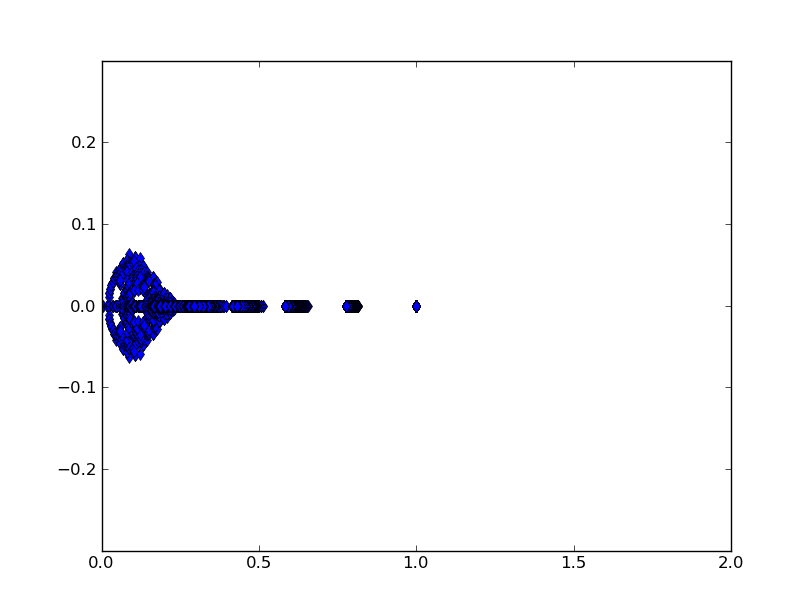
\includegraphics[width=9cm]{s8_5_5}
\caption{Spectrum of the Sweep preconditioned system}
\end{figure}
% 1.0000
% 0.0048255

% S16 : condition number : 40

\begin{figure}[H]
\centering
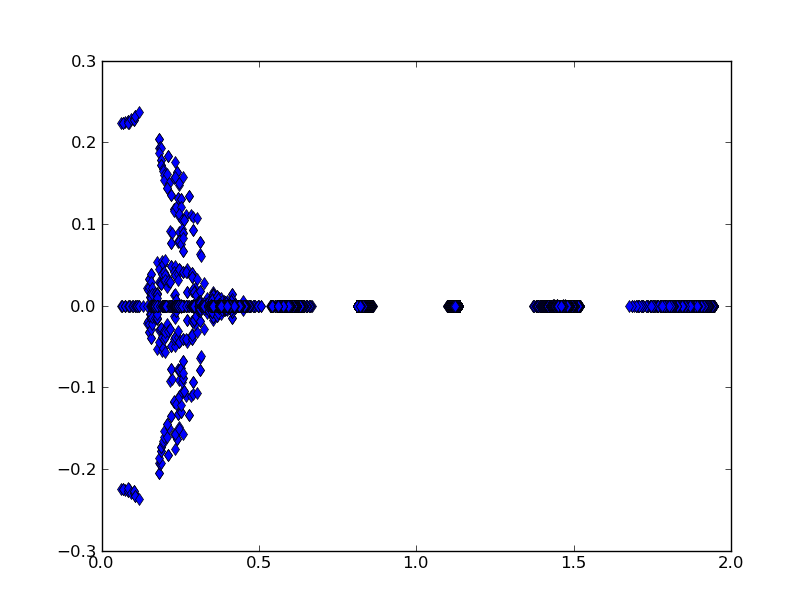
\includegraphics[width=9cm]{d_s8_5_5}
\caption{Spectrum of the DSA preconditioned system}
\end{figure}
% 1.94563117
% 0.0621324 \pm 0.224359i

% S16 : condition number : 158.9499131
% 1.98537
% 0.017012876394 \pm 0.11949429816i

\begin{figure}[H]
\centering
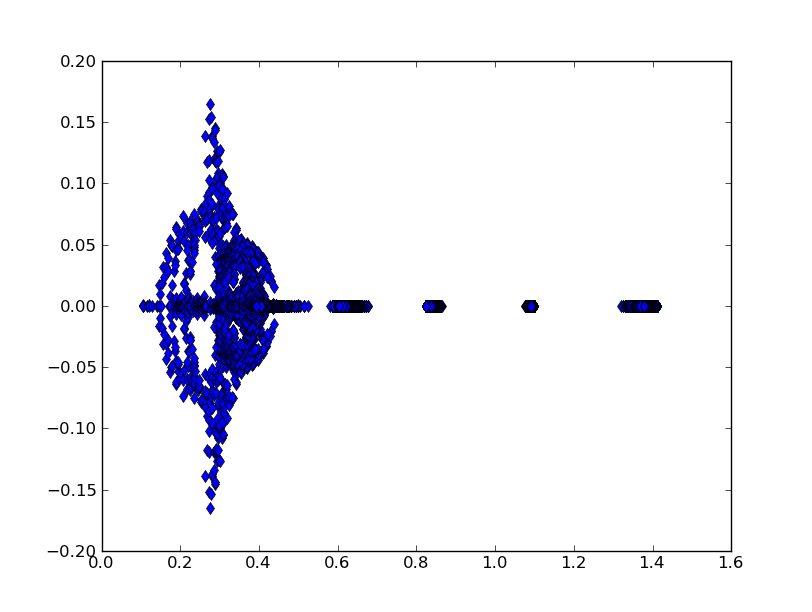
\includegraphics[width=9cm]{p_s8_5_5}
\caption{Spectrum of the Angular Multigrid with DSA preconditioned system}
\end{figure}
% 1.41172
% 0.1051087

On these figures, we can see that the DSA moves the eigenvalues away from
zero. This explains the faster convergence of GMRES with DSA preconditioning
compared to Sweep preconditioning. ANMG moves the
eigenvalues even further away than DSA and gathers them compared to DSA.
It is obvious from these figures that ANMG should converge much faster than
DSA which is what was observed in the previous tests. 

%-------------------------
%%%%%%%%%%%%%%%%%%%%%%%%%%%%%%%%%%%%%%%%%%%%%%%%%%%%%%%%%%%%%%%%%%%%%%%%%%%%%%%%%%%%
%%%%%%%%%%%%%%%%%%%%%%%%%%%%%%%%%%%%%%%%%%%%%%%%%%%%%%%%%%%%%%%%%%%%%%%%%%%%%%%%%%%%
\section{Conclusions} \label{sec:ccl}
%%%%%%%%%%%%%%%%%%%%%%%%%%%%%%%%%%%%%%%%%%%%%%%%%%%%%%%%%%%%%%%%%%%%%%%%%%%%%%%%%%%%
%%%%%%%%%%%%%%%%%%%%%%%%%%%%%%%%%%%%%%%%%%%%%%%%%%%%%%%%%%%%%%%%%%%%%%%%%%%%%%%%%%%%

In this paper, we have recalled the previous work on angular multigrid
method. For one dimensional geometry, this scheme has been proven to be very 
efficient compared to DSA. When using Fokker-Planck cross sections, the
spectral radius of the method is bounded by 0.6 while SI+DSA is bounded by 1. 
For multidimensional problems, the generalized scheme does
not show the same behavior. The angular multigrid method needs to be
stabilized
by a filter which degrades the spectral radius. The spectral radius is inferior 
to the one of DSA but it can still be arbitrary close to one. 
Unlike the previous methods which solved the $S_n$ equations using the Source 
Iteration method, we recast the angular multigrid method as a preconditioner 
for a Krylov solver. The method being stabilized with a Krylov solver, two 
versions were tested. One uses the sequence $S_n,S_{\lceil\frac{n}{2}\rceil},
\hdots,S_4,P1SA$, while the other uses the sequence $S_n,
S_{\lceil\frac{n}{2}\rceil},\hdots,S_2,DSA$.
The first sequence was proposed in \cite{multigrid_1d}, the second in 
\cite{multigrid_2d}. In \cite{multigrid_2d}, the authors did not use the first
sequence because it is known to be unstable for multidimensional problem when 
used with SI. Both sequences were tried using GMRES as Krylov solver and the 
second one was shown to be more 
efficient, i.e., the number of GMRES iterations is smaller for highly 
anisotropic medium and P1SA (PD) is more difficult to invert than
DSA (SPD). The number of GMRES iterations and the time needed
to solve the equations were compared for sweep preconditioning, DSA
preconditioning and angular multigrid-DSA preconditioning. The angular
multigrid was shown to be always faster and needed less iterations than DSA.
For highly anisotropic scattering, GMRES with angular multigrid
preconditioning is much faster than GMRES with DSA or sweep preconditioning.
The comparison of the eigenvalue spectrum of the three methods shows that 
DSA preconditioner moves the eigenvalues away from zero. The new
preconditioner moves the eigenvalues further away from zero and keeps them
closer to each others compare to DSA. This explains the
efficiency of the angular multigrid method used as a preconditioner.

%-------------------------

%%%%%%%%%%%%%%%%%%%%%%%%%%%%%%%%%%%%%%%%%%%%%%%%%%%%%%%%%%%%%%%%%%%%

\bibliographystyle{unsrt}
\bibliography{biblio}

%%%%%%%%%%%%%%%%%%%%%%%%%%%%%%%%%%%%%%%%%%%%%%%%%%%%%%%%%%%%%%%%%%%%
%%%%%%%%%%%%%%%%%%%%%%%%%%%%%%%%%%%%%%%%%%%%%%%%%%%%%%%%%%%%%%%%%%%%

\end{document}

